%! Author = sbbfti
%! Date = 10/06/2020


\section{Results}\label{sec:results}

The sensible heat loss from the skin to the environment is proportional to the difference between the \ac{t-sk} and \ac{t-op}, as shown in Equation~\ref{eq:c-r}.
Consequently, for values of \ac{t-op} higher than \ac{t-sk} the body gains sensible heat from its environment and the term \ac{c-r} becomes negative.
Figure~\ref{fig:comparison_models}A shows how the sensible heat loss estimated with the \mycite{GaggeSET} and the \mycite{Jay2015} models vary as a function of \ac{t-op}, \ac{rh}, and \ac{v}.
The former model iteratively determines \ac{t-sk}, while the latter assumes it to be constant and equal to 35~$^{\circ}$C\@.
When heat gains exceed heat losses, \mycite{GaggeSET} model estimates that some heat energy gets stored in the body and consequently \ac{t-sk} increases, as shown in Figure~\ref{fig:results_model_2}C\@.
This reduces the rate at which sensible heat gain increases as \ac{t-op} increases.

The values of \ac{w} and the respective values of \ac{w-max} for two air speeds are shown in Figure~\ref{fig:comparison_models}B\@.
The value of \ac{w-max} only varies as a function of \ac{v}.
It can be observed that the critical operative temperature at which \ac{w} equals \ac{w-max} is a inversely proportional to the value of \ac{rh}.

\begin{figure}[thb!]
    \centering
    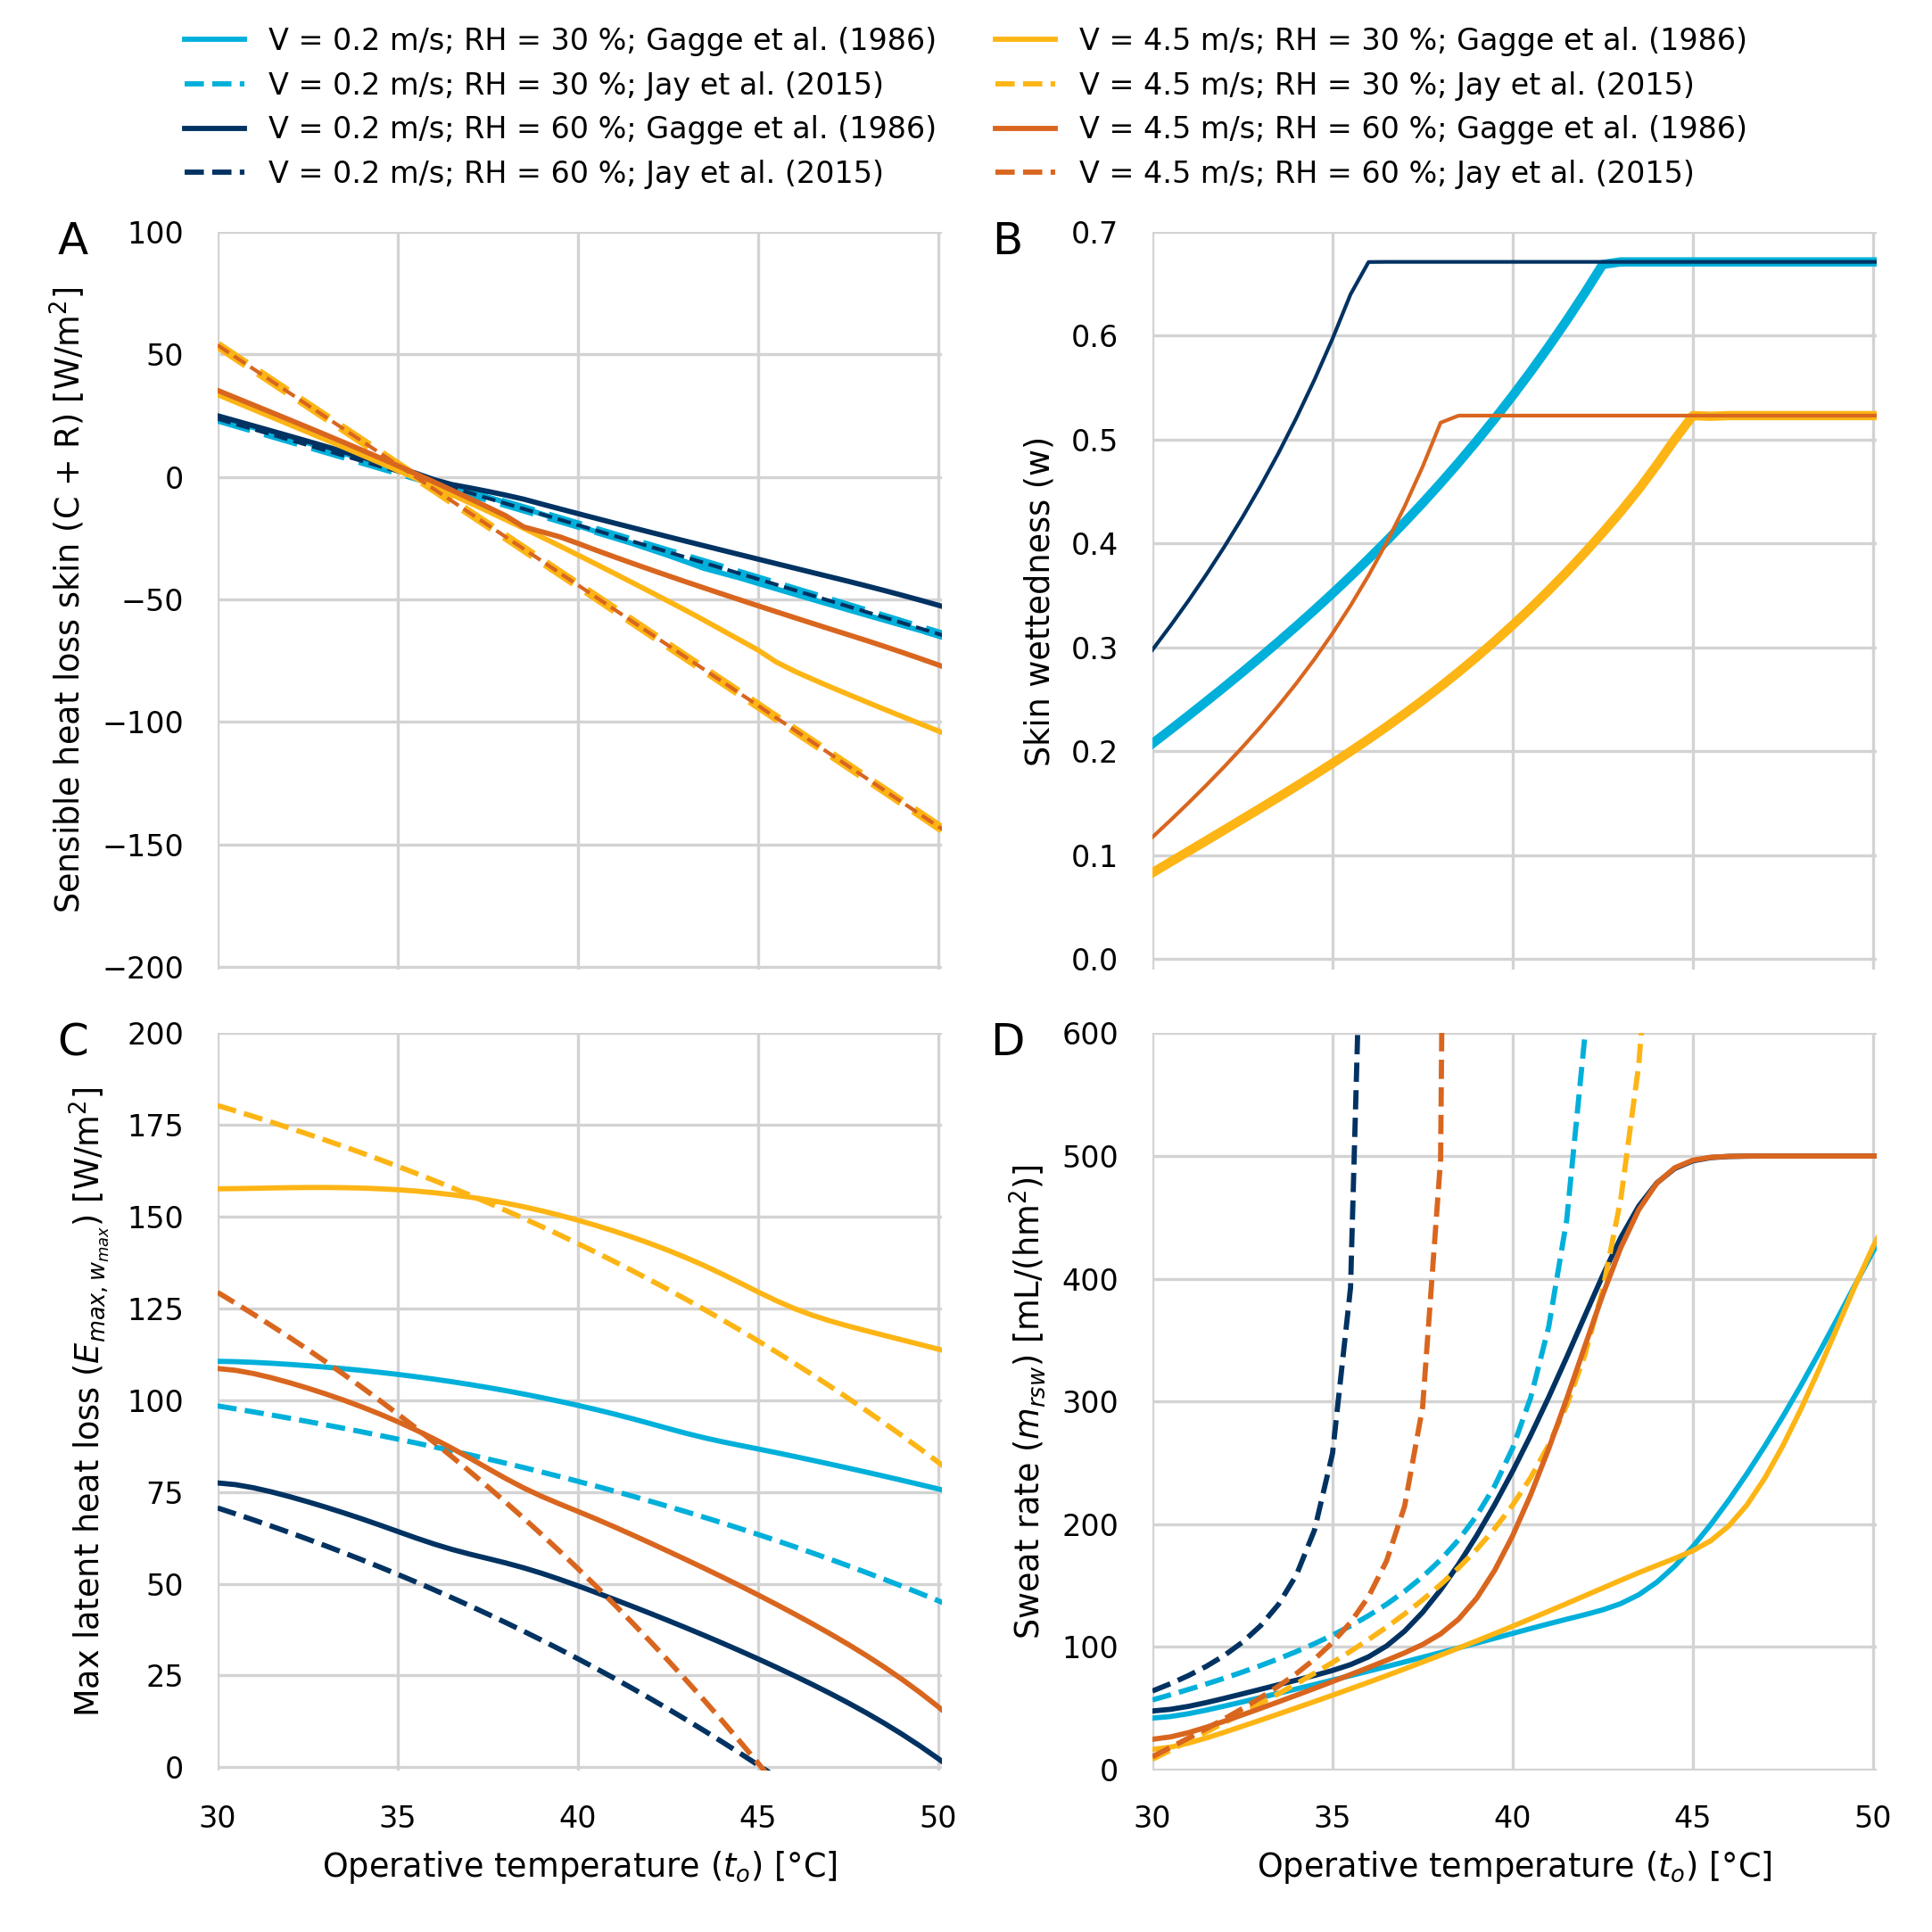
\includegraphics[width=\textwidth]{figures/comparison_models_v2.png}
    \caption{Results obtained with the the energy models proposed by \mycite{Jay2015} and \mycite{GaggeSET}.
    Each Figure shows how each parameter varies as a function of \ac{t-op} for a combination of two values of \ac{rh} and \ac{v}.
    Figure A - sensible heat loss from the skin.
    Figure B - skin wettendess.
    Figure C - Maximum latent heat loss estimated using \ac{w} = \ac{w-max}.
    Figure D - Sweat rate.}
    \label{fig:comparison_models}
\end{figure}

For \ac{t-op} higher than \ac{t-sk}, the negative effect that an increase in \ac{v} has on sensible heat gain is compensated by a greater increase in the \acf{e-sk} that the body can dissipate towards the surrounding environment.
For example, when \ac{t-op}~=~45~$^{\circ}$C and \ac{rh}~=~30~\%, an increase in \ac{v} from 0.2 to 4.5~m/s increases the sensible heat gains (\acs{c-r}) by 29 W/m\textsuperscript{2} while increasing \ac{e-sk} by 45~W/m\textsuperscript{2}, hence, increasing \ac{v} has a net positive effect.

Figure~\ref{fig:comparison_models}C shows the values of \ac{e-max} estimated by replacing \ac{w} in Equation~\ref{eq:latent-skin} with \ac{w-max}.
The value of \ac{e-max} decreases as the \ac{t-op} increases since \ac{p-a} grows more rapidly than \ac{p-sk}.
For a set combination of \ac{v} and \ac{t-op} the value of \ac{e-max} decreases as the value of \ac{rh} increases since humid air has a higher \ac{p-a} than dry air.
The reduction in \ac{e-max} estimated by our model is lower than the one estimated by \mycite{Jay2015} since an increase in \ac{t-sk} elevates the vapor pressure gradient between the skin and the surrounding environment.

The \acf{m-sweat} is shown in Figure~\ref{fig:comparison_models}D\@.
The difference between the results obtained with the two heat balance models can be attributed to the fact that \citeauthor{Jay2015} calculate the value of \ac{m-sweat} as a function of the required latent energy that the body should in theory dissipate to achieve thermal neutrality.
On the other hand, \citeauthor{GaggeSET} calculate the value of \ac{m-sweat} as a function of regulatory signals and they assume that \ac{m-sweat} cannot exceed 500~mL/h.
% todo check this since it does not convince me

\begin{figure}[thb!]
    \centering
    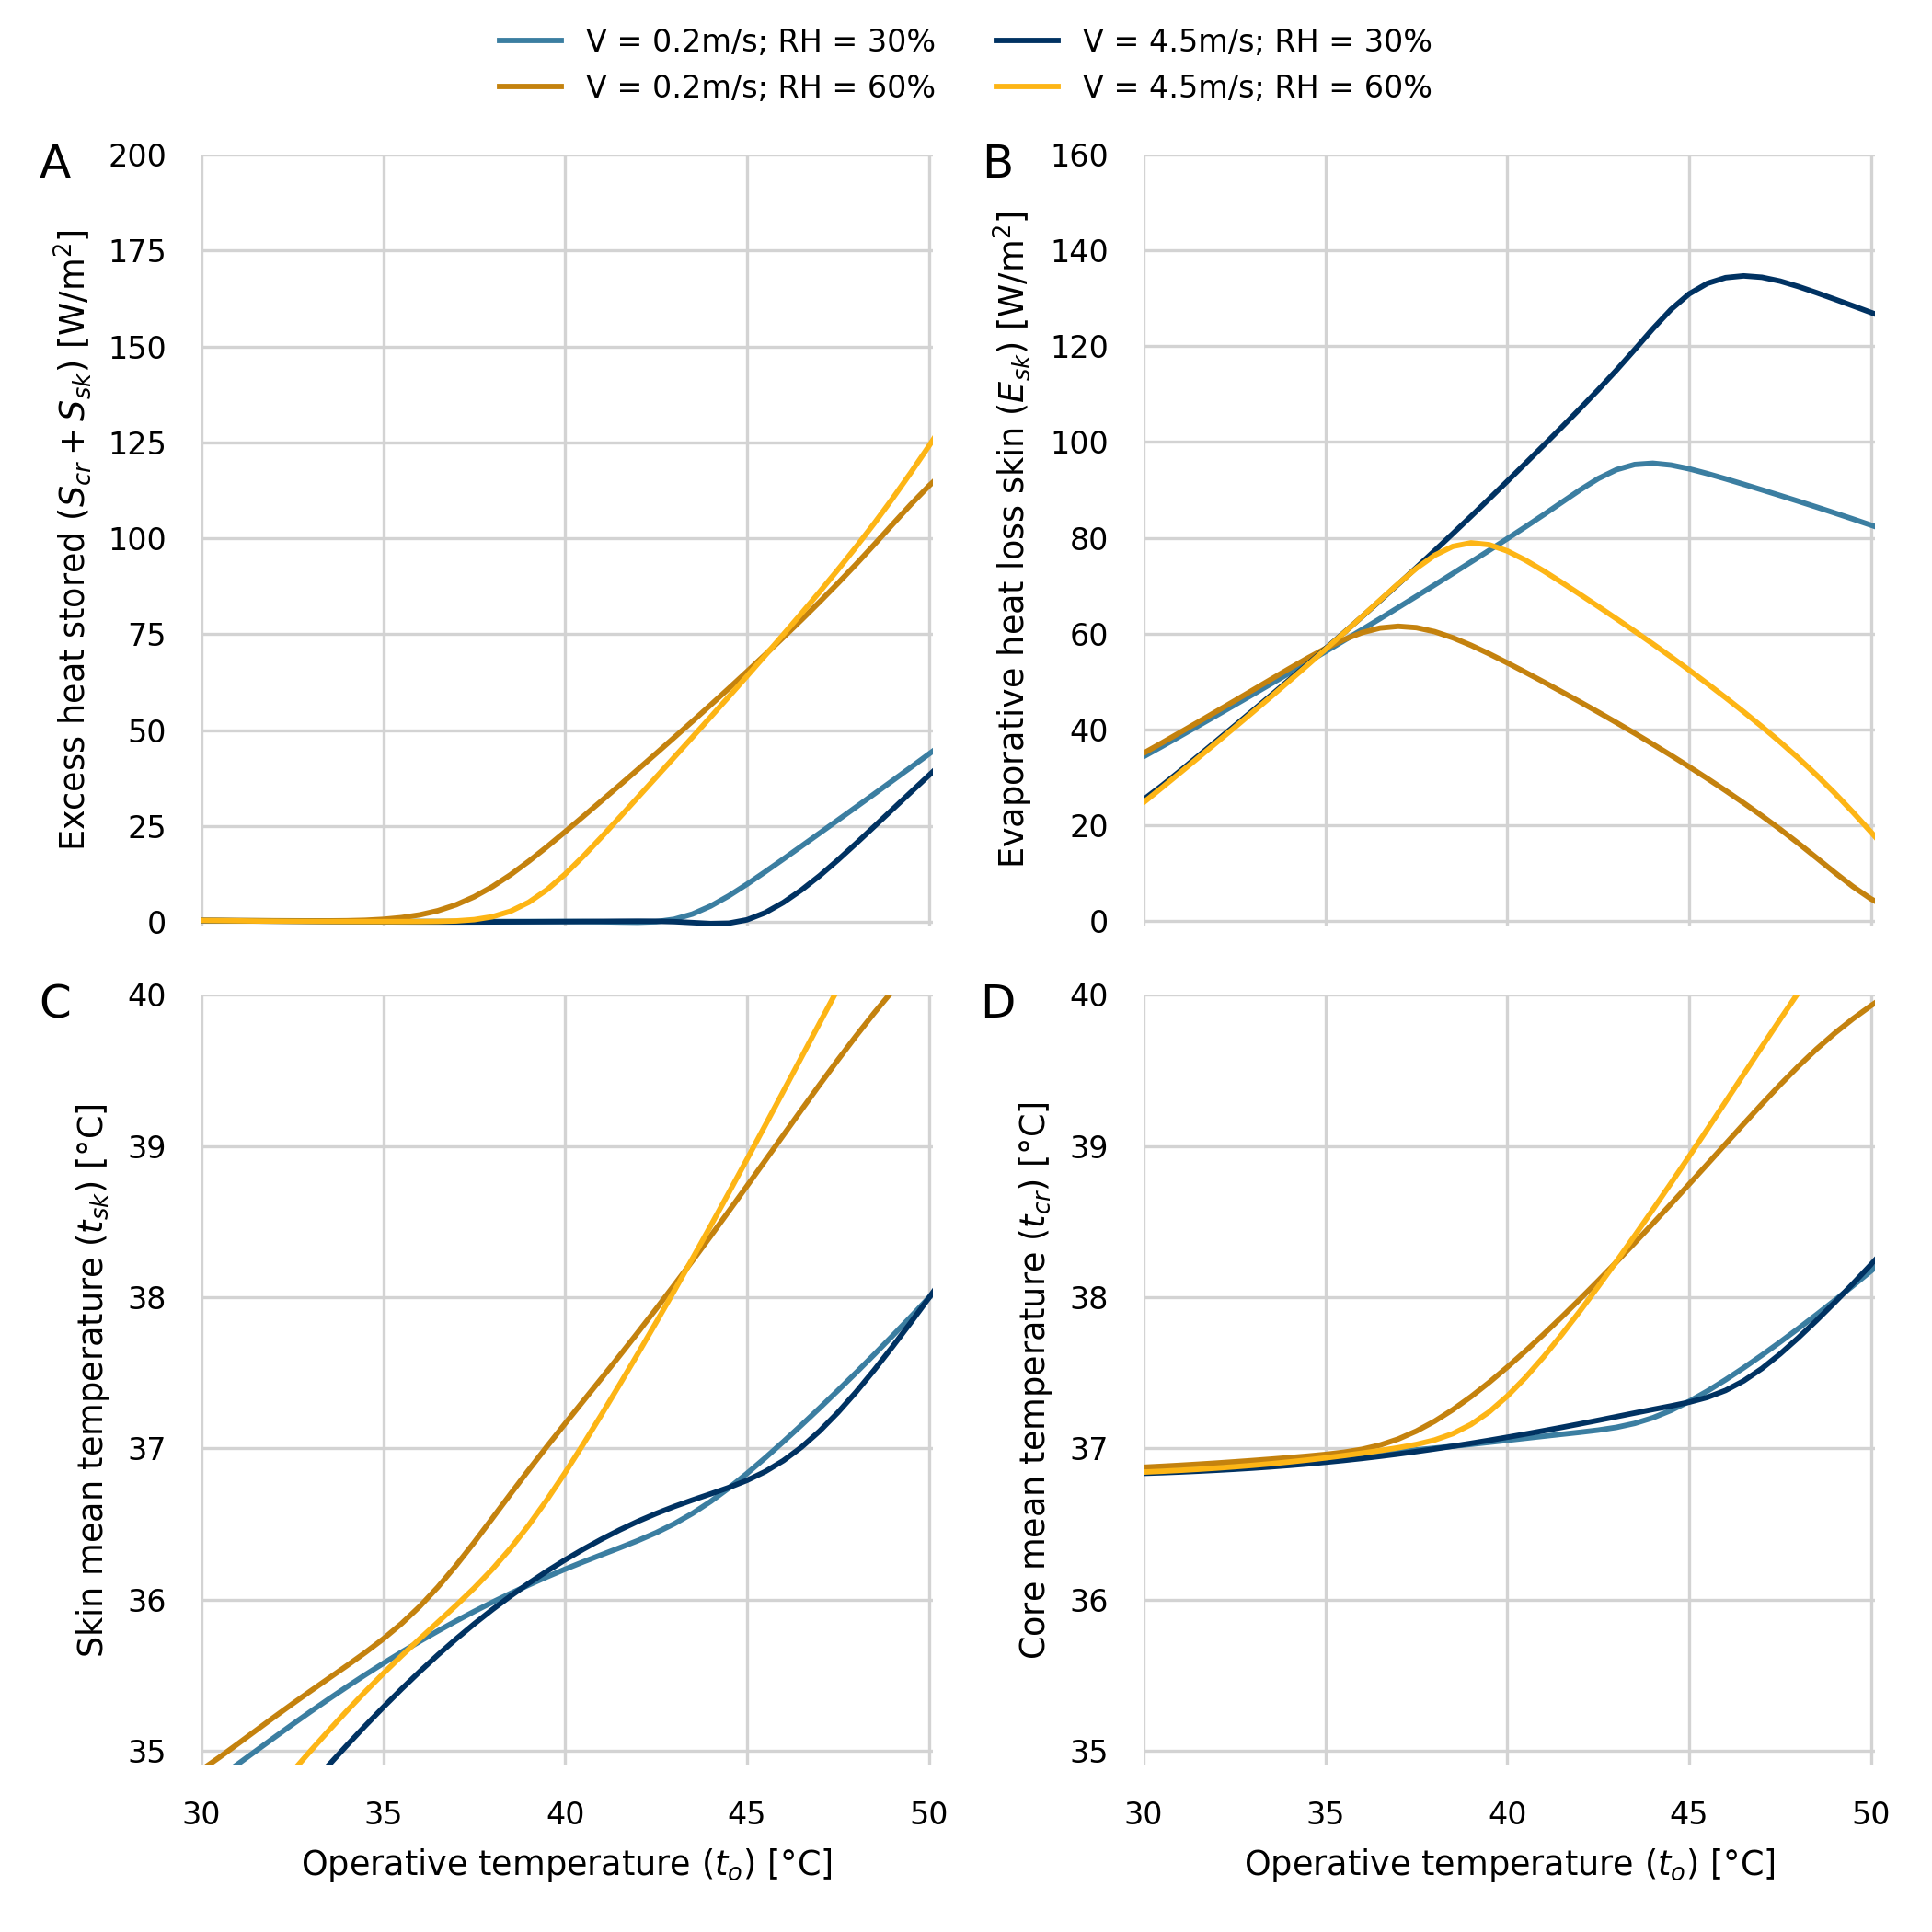
\includegraphics[width=\textwidth]{figures/results_model_2.png}
    \caption{Caption}
    \label{fig:results_model_2}
\end{figure}

The excess heat stored in the human body (\acs{s-cr} + \acs{s-sk}), \ac{t-sk}, and \ac{t-cr} are shown in Figure~\ref{fig:results_model_2}A, ~\ref{fig:results_model_2}C, and ~\ref{fig:results_model_2}D, respectively.
When the body cannot longer dissipate exogenous and endogenous heat gains, the excess heat gets stored in the human body causes \ac{t-sk} and \ac{t-cr} to raise.

The combination of \ac{t-op}, \ac{rh}, and \ac{v} at which heat strain would start to occur is presented in Figure~\ref{fig:comparison_air_speed}.
Each line demarcates the region in which thermal stress is estimated to occur and not all individuals would be able to compensate for endogenous and exogenous heat gains.
The Figure shows the results obtained with both the \mycite{GaggeSET} and the \mycite{Jay2015} models.
For a specific value of \ac{v}, the maximum \ac{t-op} at which cardiovascular strain is estimated to occur decreases as the value of \ac{rh} increases.
In addition, it can be observed that for a specific value of \ac{rh}, as the value of \ac{v} increases the overall increase in the maximum critical temperature rapidly decreases.
For example, in an environment with \ac{rh}~=~60~\%, increasing \ac{v} from 0.2~m/s to 0.8~m/s then to 4.5~m/s lead to an increase of the critical temperature of approximately 2.3~$^{\circ}$C and 0.8~$^{\circ}$C, respectively.

In addition, in Figure~\ref{fig:comparison_air_speed} we are presenting the results obtained by \mycite{Morris2019} who studied whether the use of fans (\ac{v}~=~2.0~m/s) is beneficial in two environmental conditions hot and humid (green dot) and hot and dry (red dot).
The black dashed lines are isoenthalpic lines passing through the conditions studied by \mycite{Morris2019}.
Our results show that if electric fans are used in hot and dry conditions heat strain would occur at relative low enthalpy values.
This can be explained by the fact that the value of skin blood flow increases proportionally to the value of \ac{v}.
Our model, appears to slightly underestimate this effect since in `theory' electrical fans should not be used for \ac{rh} lower than 10~\% and \ac{t-db} higher than 49~$^{\circ}$C\@, which is where the gray solid line intercepts the yellow line.
It should, however, be noted that, as previously mentioned in the Introduction Section, the hot and dry condition has a lower enthalpy than the hot and humid one, hence, evaporative cooling technologies can be used to reduce skin blood flow and avoid heat strain.
Evaporative cooling is an isoenthalpic process that causes a drop in \ac{t-db} proportional to the sensible heat drop and an increase in humidity ratio proportional to the latent heat gain.
Evaporative cooling can be achieved by spraying water in the air or even by placing wet towels near the electric fan.

\begin{figure}[thb!]
    \centering
    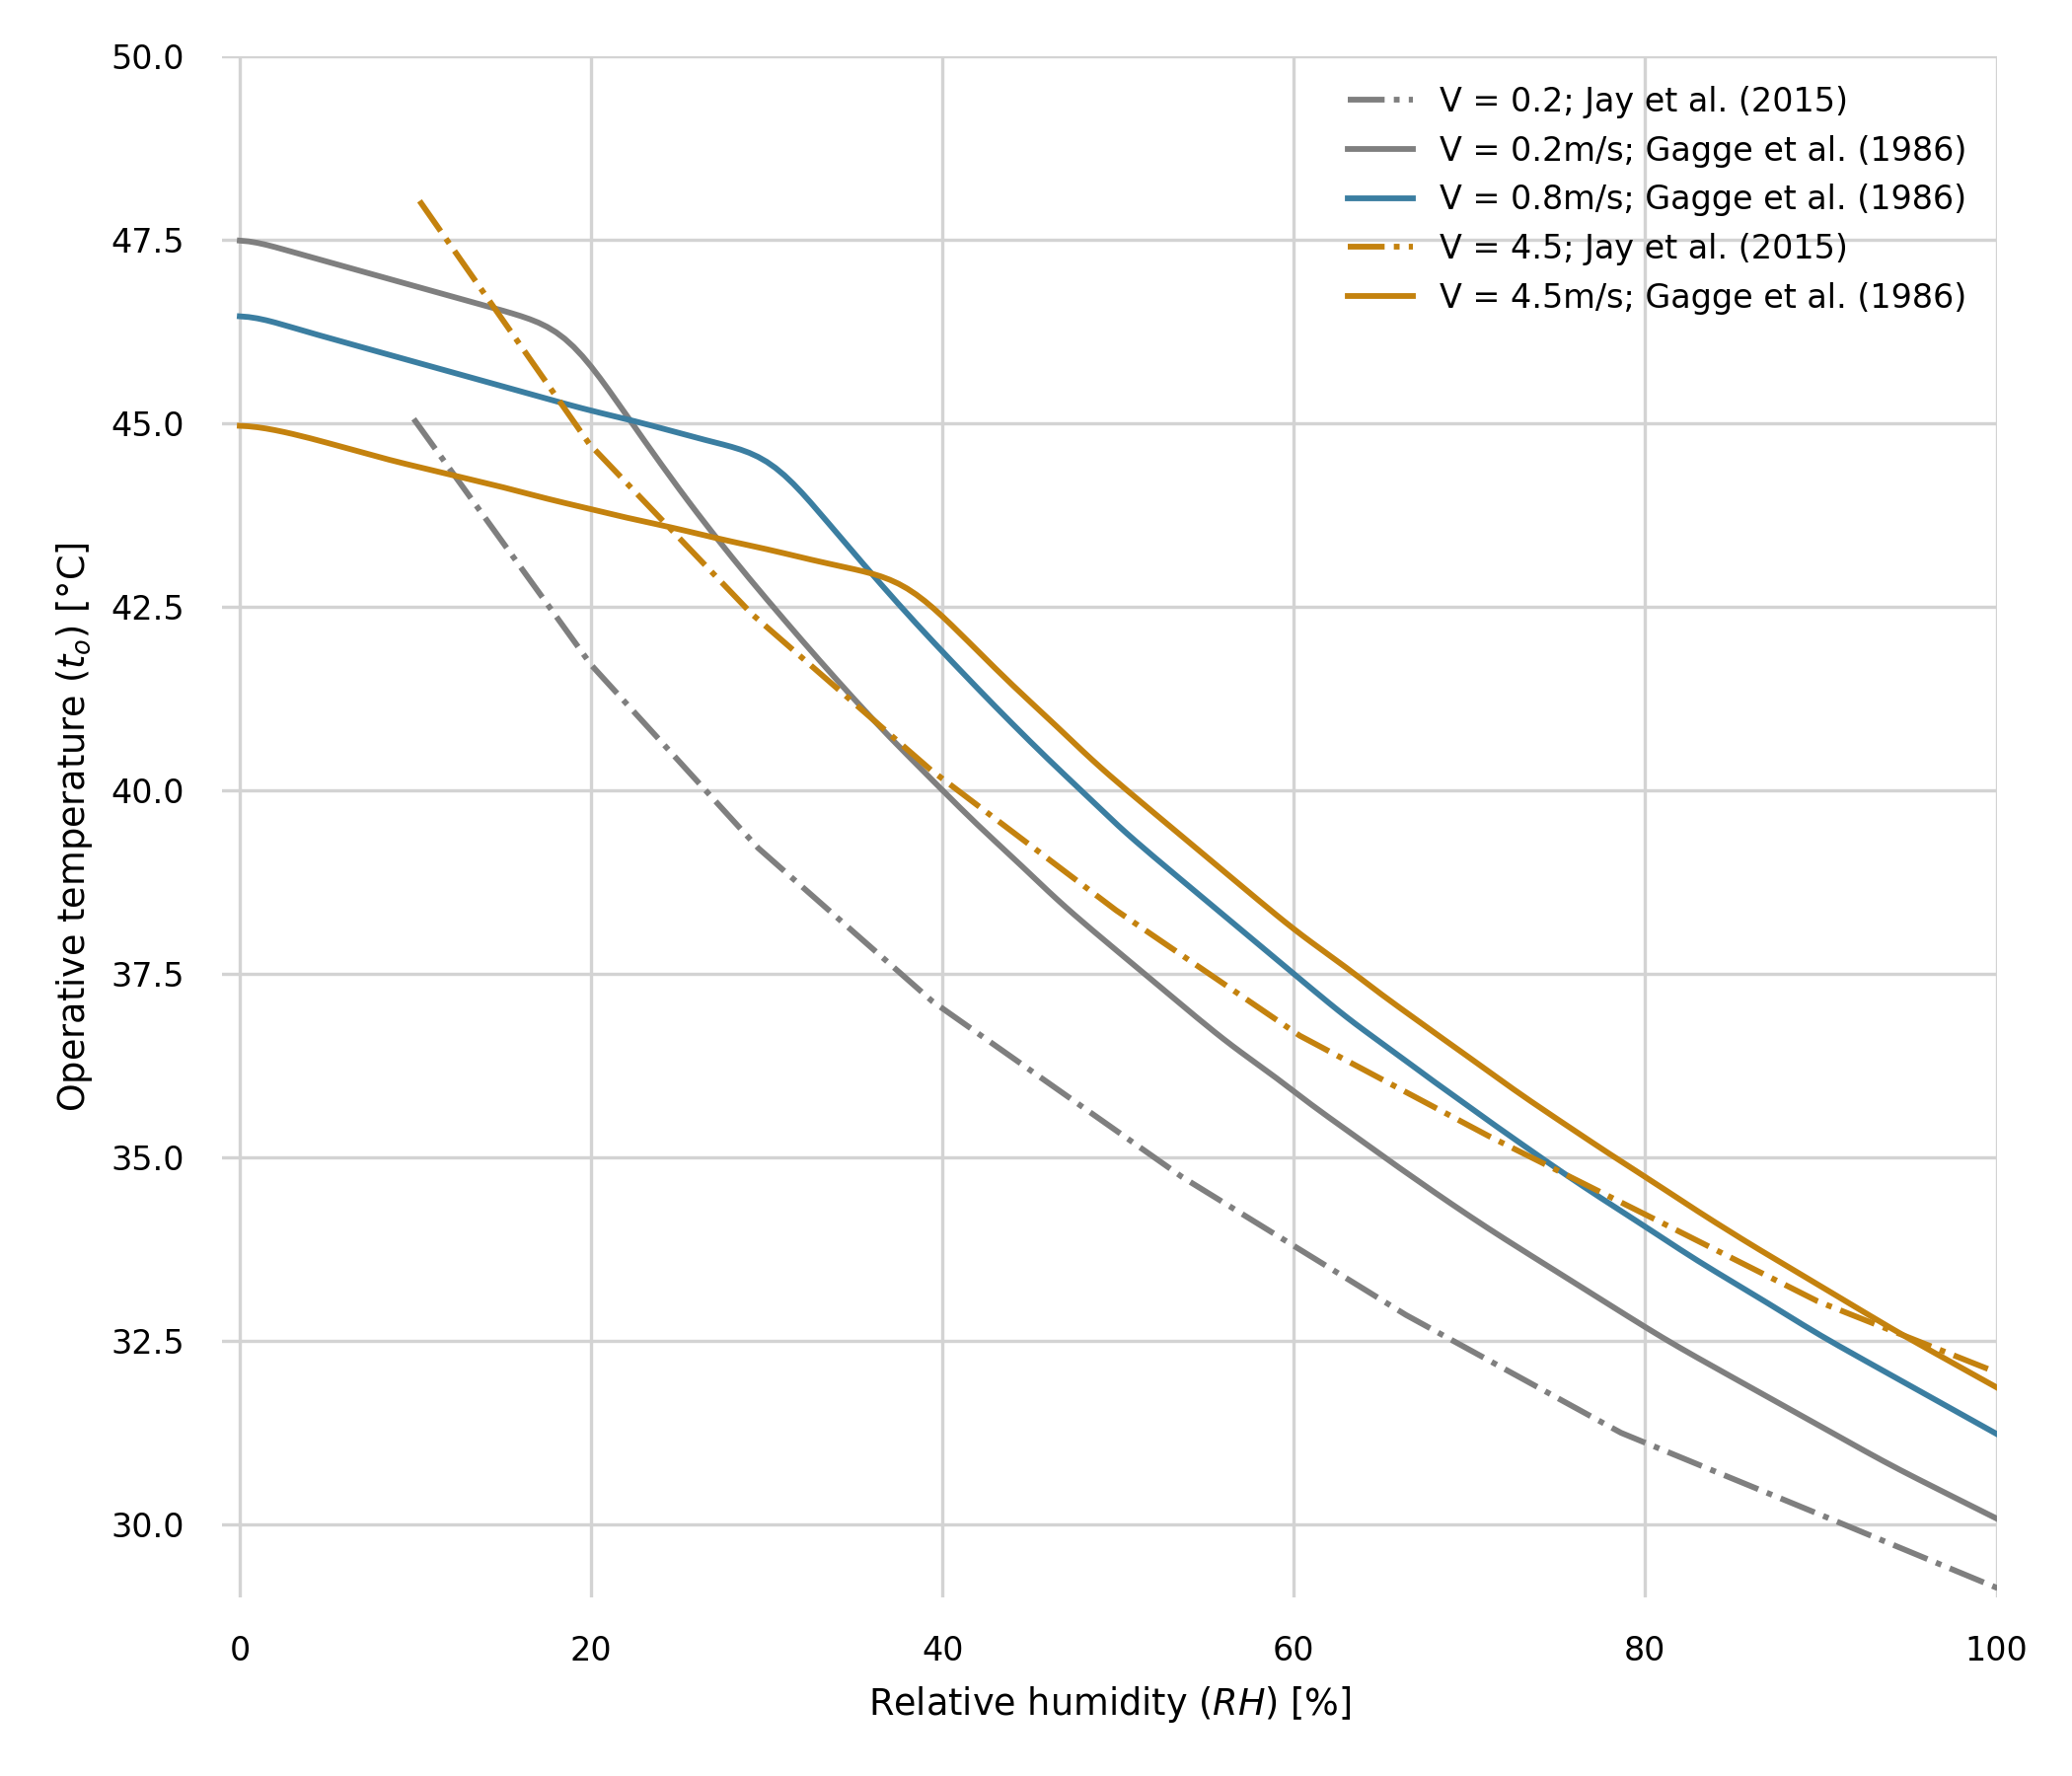
\includegraphics[width=\textwidth]{figures/comparison_air_speed.png}
    \caption{Compares the results between the \mycite{GaggeSET} and the \mycite{Jay2015} models.
    The solid and dash dotted lines demarcate the point above which heat stress is expected to occur.
    The dashed lines are isoenthalpic lines, which show the enthalpy of the two conditions studied by \mycite{Morris2019}}
    \label{fig:comparison_air_speed}
\end{figure}

To better understand how personal factors would impact the body ability to dissipate heat we calculate when heat strain would occur for different combinations of \ac{met} and \ac{clo}.
Results for people wearing light summer clothing (walking shorts, short-sleeve shirt and sandals, \acs{clo} = 0.36 clo), and office summer clothing (trousers, short-sleeve shirt, and closed shoes \acs{clo} = 0.5 clo) who are either seated reading or writing (\ac{met} = 1.0 met) or standing relaxed (\ac{met} = 1.2 met) are shown in Figure~\ref{fig:met_clo}.
As expected, decreasing both \ac{met} and \ac{clo} has a net positive effect since it reduces both heat gains and thermal resistance.

\begin{figure}[thb!]
    \centering
    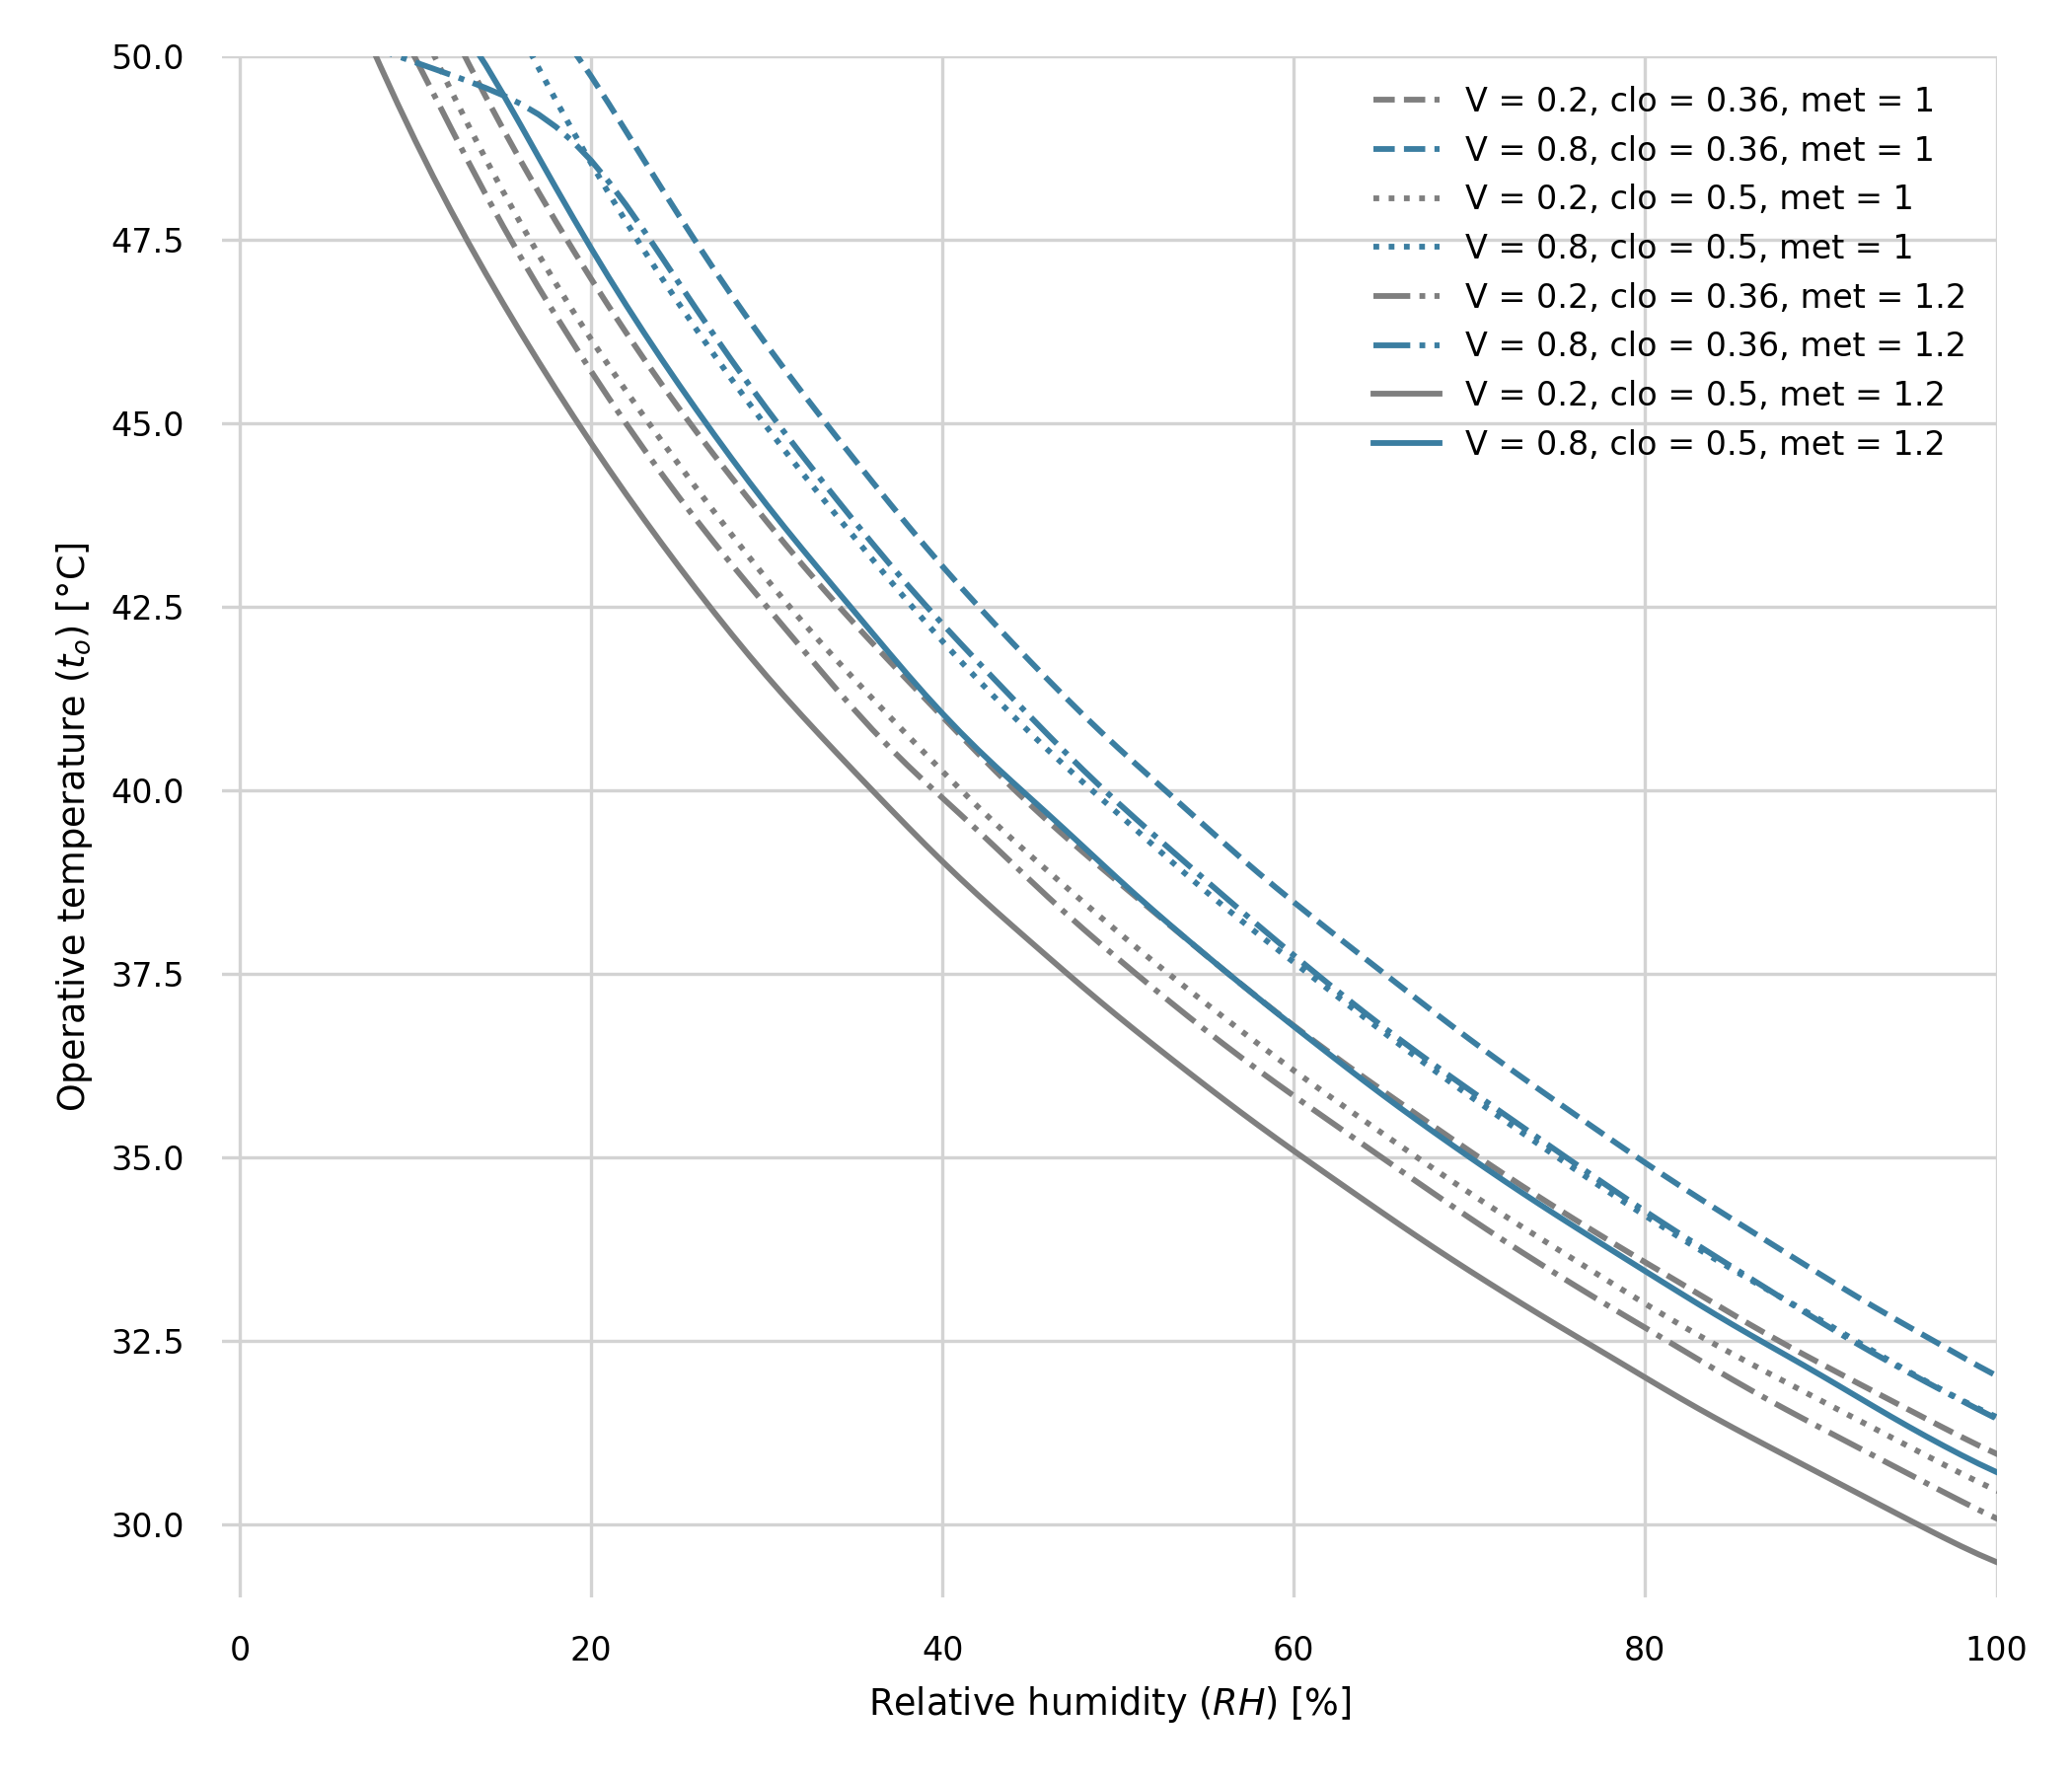
\includegraphics[width=\textwidth]{figures/met_clo.png}
    \caption{Each line demarcates how different combinations of personal factors (e.g., \ac{met}, \ac{clo}) and environmental factors affect the point above which the body cannot longer dissipate all the endogenous and exogenous heat gains}
    \label{fig:met_clo}
\end{figure}

The environmental conditions above which the use of elevated air speeds would actually be detrimental for the great majority of people is shown in Figure~\ref{fig:energy_storage_delta}.
We used a red filling to highlight the region in which electrical fans should not be used, while we used a green background to depict when elevated air speed can safely be used to cool the human body.
We used a blue background to show the area in which fans are effective tool to prevent heat strain only if are used in combination with evaporative cooling technologies.
We also plotted the lines above which thermal strain is expected to occur (see Figure~\ref{fig:comparison_air_speed} fro more details).
For a specific value of \ac{rh}, as the value of \ac{v} increases the critical temperature at which thermal strain would occur also increases, however, at the same time the temperature above which fans should not be used also decreases by a greater amount.

We used a scatter plot to visualize the maximum extreme weather conditions recorded worldwide in more than 5000 stations.
Each dot represents the most extreme heat event recorded in each location.
Based on the climate data obtained from the 2017 ASHRAE Handbook--Fundamentals we determined that in approximately 67~\% of the locations thermal strain should not occur even without air movement, however, this number increases to 87~\% and 92~\% when \ac{v} is increased to 0.8~m/s and 4.5~m/s, respectively.
The use of fans during heatwaves would, therefore, be beneficial in the great majority of the locations worldwide.
With the exception of 23 locations where the use of \ac{v} higher than 0.8~m/s would be detrimental for the human body, and 7 locations where elevated air movement should not be used in any scenario.

% https://advances.sciencemag.org/content/6/19/eaaw1838

% todo report estimated sweat heat lossess too, either using a table or a heatmap

\begin{figure}[thb!]
    \centering
    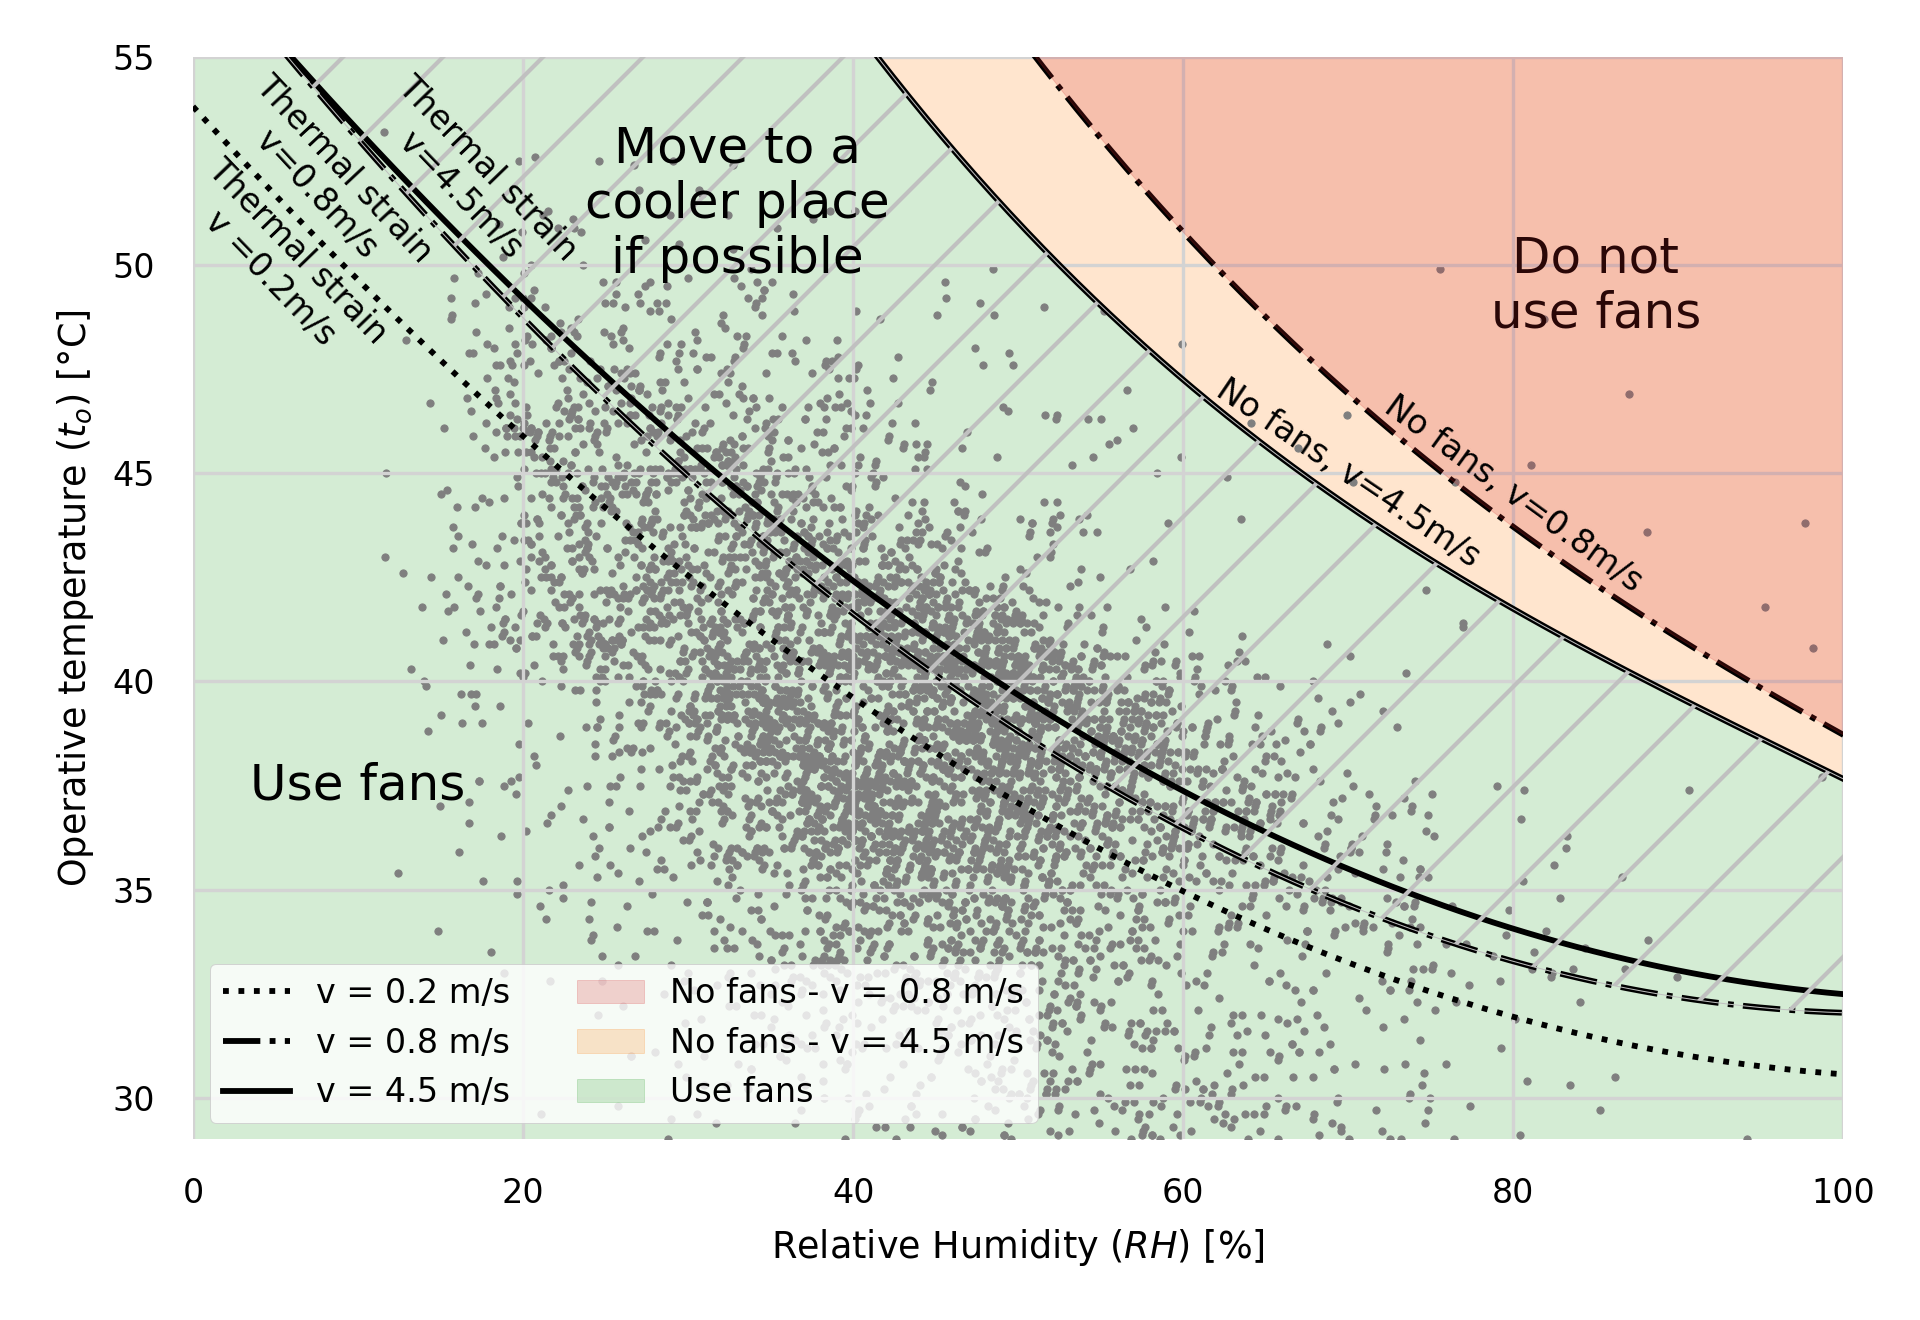
\includegraphics[width=\textwidth]{figures/use_fans.png}
    \caption{The green area shows the environmental conditions in which the use of fans is beneficial since they provide additional cooling to the human body.
    In the hatched area, while the use of fans it is still beneficial, people are most likely to suffer from heat stress.
    Finally the red area demarcates the region in which electrical fans should not be used.
    The dots show the maximum extreme climate conditions recorded over the last 10 years in more than 5000 locations worldwide.
     These results were calculated assuming \ac{t-r} = \ac{t-db}, \ac{clo} = 0.5~clo, \ac{met} = 1.0~met.}
    \label{fig:energy_storage_delta}
\end{figure}


